\documentclass[obeyspaces,spaces,hyphens,handout]{beamer}
\usepackage[spanish]{babel}
\usepackage{pst-node}
\usepackage{fontspec}
\usepackage{graphicx}

%\mode<presentation>

\begin{document}
\title{Bases de datos no tradicionales - clase 2}
\author{Felipe Gorostiaga - Guido Martínez}
\institute{Bases de datos avanzadas, LCC}

\begin{frame}
  \titlepage
\end{frame}

\AtBeginSection{\frame{\sectionpage}}

\setbeamertemplate{section page}
{
	\begin{centering}
	\begin{beamercolorbox}[sep=12pt,center]{part title}
	\usebeamerfont{section title}\bf{\insertsection}\par
	\end{beamercolorbox}
	\end{centering}
}

\newcommand{\dquote}{\texttt{\char`\"}}

\section{XML}

\begin{frame}
\frametitle{Introducción}
\begin{itemize}

\item	XML es un lenguaje de ``markup'', o sea, permite estructurar documentos
	y agregar metadatos de manera que sea sintáctimente distinguible del
	contenido.
	\pause

\item	Fue diseñado por el W3C con los objetivos de:
\begin{itemize}
	\item	Que sea fácilmente usable a través de toda la internet
	\item	Que pueda soportar distintos tipos de uso y aplicaciones
	\item	Que sea fácil escribir programas que usen documentos XML
	\item	Que sea legible por un humano
	\item	etc...
\end{itemize}
\pause

\item	En otras palabras, que sea {\it el} lenguaje estándar para intercambio
	de datos.
\pause

\item	Es conceptualmente un árbol, con una única raíz.
\pause

\item	El árbol no tiene una estructura predefinida (XML es de alguna manera
	un metalenguaje) y es lo más genérico posible. Cada nodo (usualmente
	llamado elemento) tiene:
	\pause
\begin{itemize}
	\item	Un nombre, que usualmente representa el ``tipo''
		del elemento.
		\pause
	\item	Opcionalmente, una lista de atributos.
		\pause
	\item	Su contenido, que puede estar compuesto por
		mas elementos.
\end{itemize}

\end{itemize}
\end{frame}

\begin{frame}
\frametitle{Ejemplos - 1}
\footnotesize
\texttt{<note>						\\
	~~<to>Tove</to>					\\
	~~<from>Jani</from>				\\
	~~<heading>Reminder</heading>			\\
	~~<body>Don't forget me this weekend!</body>	\\
	</note>
}
\end{frame}

\begin{frame}
\frametitle{Ejemplos - 2}
\footnotesize
\texttt{<CATALOG>				\\
	~~<CD>					\\
	~~~~<TITLE>Empire Burlesque</TITLE>	\\
	~~~~<ARTIST>Bob Dylan</ARTIST>		\\
	~~~~<COUNTRY>USA</COUNTRY>		\\
	~~~~<COMPANY>Columbia</COMPANY>		\\
	~~~~<PRICE>10.90</PRICE>		\\
	~~~~<YEAR>1985</YEAR>			\\
	~~</CD>					\\
	~~<CD>					\\
	~~~~<TITLE>Hide your heart</TITLE>	\\
	~~~~<ARTIST>Bonnie Tyler</ARTIST>	\\
	~~~~<COUNTRY>UK</COUNTRY>		\\
	~~~~<COMPANY>CBS Records</COMPANY>	\\
	~~~~<PRICE>9.90</PRICE>			\\
	~~~~<YEAR>1988</YEAR>			\\
	~~</CD>					\\
	</CATALOG>
}
\end{frame}

\begin{frame}
\frametitle{Ejemplos - 3}
\footnotesize
\texttt{<CATALOG>				\\
	~~<CD>					\\
	~~~~<TITLE>Empire Burlesque</TITLE>	\\
	~~~~<ARTIST>Bob Dylan</ARTIST>		\\
	~~~~<COUNTRY>USA</COUNTRY>		\\
	~					\\
	~~~~<PRICE>10.90</PRICE>		\\
	~					\\
	~~</CD>					\\
	~~<CD>					\\
	~~~~<TITLE>Hide your heart</TITLE>	\\
	~~~~<ARTIST>Bonnie Tyler</ARTIST>	\\
	~~~~<COUNTRY>UK</COUNTRY>		\\
	~~~~<COMPANY>CBS Records</COMPANY>	\\
	~					\\
	~~~~<YEAR>1988</YEAR>			\\
	~~</CD>					\\
	</CATALOG>
}
\end{frame}

\newcommand{\dquote}{\texttt{\char`\"}}

\begin{frame}
\frametitle{Ejemplos - 4}
\footnotesize
\texttt{<td style=\dquote line-height:1.35em;\dquote>		\\
	~~<a href=\dquote /wiki/Markup\_language\dquote ~
		title=\dquote Markup language\dquote>		\\
	~~~~Markup language					\\
	~~</a>							\\
	</td>
}
\end{frame}

\begin{frame}
\frametitle{Parseo}
\begin{itemize}
	\item	Existen muchisímas librerías que parsean XML, por lo cual
		adaptar una aplicación existente a usar XML suele ser fácil
		(nunca tenemos que preocuparnos por parsearlo).
		\pause

	\item	Interpretar el XML es trabajo de la aplicación en cuestión
		(ya que la definición de XML no acarrea significado).
\end{itemize}
\end{frame}

\section{XSD}

\section{XSLT}

\begin{frame}
\frametitle{Transformación automática}
\begin{itemize}
\item	XSLT es otra propuesta del W3C. Es un lenguage para
	representar transformaciones de XML a otros lenguajes
	(incluído XML).
	\pause

\item	Definiendo las reglas podemos lograr algo que transforme
	de datos XML a, por ejemplo, una página web que los muestre.
\end{itemize}
\end{frame}

\begin{frame}
\centering
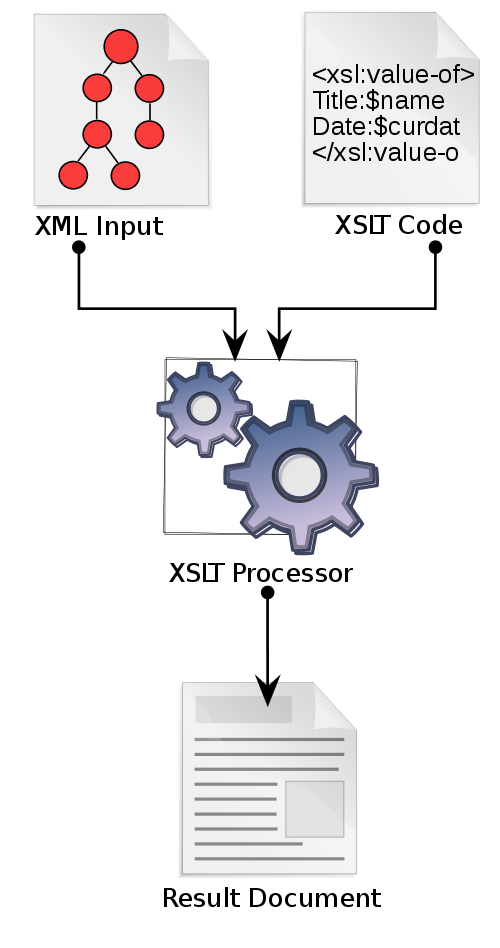
\includegraphics[scale=0.25]{xslt}
\end{frame}

\begin{frame}
\frametitle{Ejemplo - Documento original}

\footnotesize
\texttt{<persons>					\\
	~~<person username='JS1'>			\\
	~~~~<name>John</name>				\\
	~~~~<family-name>Smith</family-name>		\\
	~~</person>					\\
	~~<person username='MI1'>			\\
	~~~~<name>Morka</name>				\\
	~~~~<family-name>Ismincius</family-name>	\\
	~~</person>					\\
	</persons>}
\end{frame}
\begin{frame}
\frametitle{Ejemplo - Código XSLT}

\footnotesize
\texttt{<xsl:stylesheet version='1.0'>			\\
	~~<xsl:output method='xml' indent='yes'/>	\\
	~						\\
	~~<xsl:template match='/persons'>		\\
	~~~~<root>					\\
	~~~~~~<xsl:apply-templates select='person'/>	\\
	~~~~</root>					\\
	~~</xsl:template>				\\
	~						\\
	~~<xsl:template match='person'>			\\
	~~~~<name username='{@username}'>		\\
	~~~~~~<xsl:value-of select='name' />		\\
	~~~~</name>					\\
	~~</xsl:template>				\\
	</xsl:stylesheet>
	}
\end{frame}

\begin{frame}
\frametitle{Ejemplo - Resultado}

\footnotesize
\texttt{<root>						\\
	~~<name username='JS1'>John</name>		\\
	~~<name username='MI1'>Morka</name>		\\
	</root>
}
\end{frame}

\section{JSON}
\begin{frame}
\frametitle{Introducción}
\begin{itemize}
\item	JSON es un formato de intercambio de datos liviano, desarrollado con el objetivo de minimizar el overhead y ser fácilmente legible y editable tanto por máquinas como por seres humanos.
		\pause
\item	Está basado en un subconjunto del estándar de JavaScript, y esto es lo que le da su nombre: ``JavaScript Object Notation''.
\end{itemize}
\end{frame}

\begin{frame}
\frametitle{Un JSON bien formado}
\begin{itemize}
\item	JSON se construye a partir de dos estructuras:
		\pause
\begin{itemize}
		\item	Una colección de pares clave -> valor (al estilo de un objeto ó record ó struct ó diccionario ó tabla hash ó arreglo asociativo en los lenguajes de programación).
				\pause
		\item	Una lista ordenada de valores (al estilo de un array ó vector ó lista ó secuencia en los lenguajes de programación).
\end{itemize}
\end{itemize}
\end{frame}

\begin{frame}
\frametitle{Un JSON bien formado}
\begin{itemize}
\item	En JSON se representan de las siguientes maneras, respectivamente:
		\pause
\begin{itemize}
		\item	Un objeto comienza con una llave izquierda \texttt{\{} y termina con una llave derecha \texttt{\}}. Cada clave es seguida por dos puntos \texttt{:}, y los pares clave -> valor se separan mediante una coma \texttt{,}. \\
				\pause
				Gráficamente: \\
				\begin{figure}
				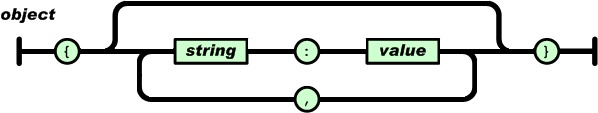
\includegraphics[scale=0.4]{JSONObject}
				\end{figure}
				\pause
		\item	Un arreglo comienza con un corchete izquierdo \texttt{[} y finaliza con un corchete derecho \texttt{]}. Los elementos del arreglo son separados por coma \texttt{,}. \\
				\pause
				Gráficamente: \\
				\begin{figure}
				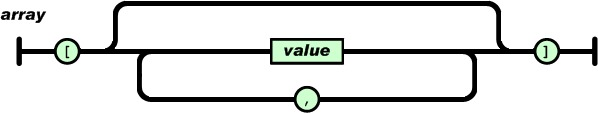
\includegraphics[scale=0.4]{JSONArray}
				\end{figure}
\end{itemize}
\end{itemize}
\end{frame}

\begin{frame}
\frametitle{Un JSON bien formado}
\begin{itemize}
\item	Finalmente, se especifica el tipo de los valores que pueden estar ligados a una clave. Estos son:
\begin{itemize}
	\item	cadenas de texto
	\item	números
	\item	objetos (ítems 'a' de las diapositivas anteriores)
	\item	arreglos (ítems 'b' de las diapositivas anteriores)
	\item	true (literal booleano)
	\item	false (literal booleano)
	\item	null
\end{itemize}
\pause
\item Gráficamente: \\
		\begin{figure}
		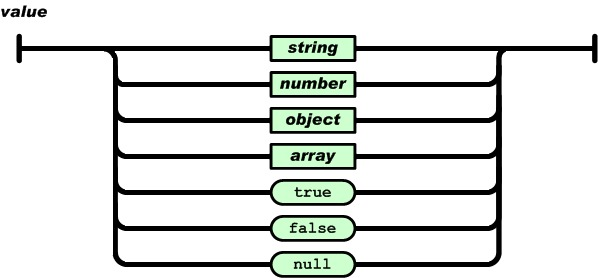
\includegraphics[scale=0.4]{JSONValue}
		\end{figure}
\end{itemize}
\end{frame}

\begin{frame}
\frametitle{JSON vs XML}
\end{frame}

\section{Key-value stores}
\begin{frame}
\frametitle{Introducción}
\begin{itemize}
\item	Las bases de datos clave $\rightarrow$ valor están diseñadas para almacenar arreglos asociativos, también conocidos como tablas hash o diccionarios. \pause
\item	Únicamente permiten persistir pares clave $\rightarrow$ valor, y recuperar un valor cuando se provee su clave. \pause
\item	Para la base de datos, los valores son objetos oscuros, que no sabe interpretar. \pause
\item	Esta simplicidad los hace una alternativa muy eficiente, fácilmente implementable, versátil y escalable ante las bases de datos relacionales, aunque para aplicaciones grandes y complejas, probablemente sea mejor optar por alguna de sus extensiones: \pause
\begin{itemize}
		\item	Bases de datos orientadas a columnas \pause
		\item	Bases de datos de documentos.
\end{itemize}
\end{itemize}
\end{frame}

\begin{frame}
\frametitle{Uso y ejemplos}
\begin{itemize}
	\item	Son la versión mas simple de bases de datos NoSQL,
		desde el punto de vista de su uso (su API). El cliente
		sólo puede hacer \textit{get}, \textit{put} o
		\textit{remove} sobre \textit{buckets}.
		\pause

	\item	Algunos ejemplos son: Riak, MemcacheDB, Redis y
		DynamoDB de Amazon.
		\pause

	\item	Redis, en particular, puede almacenar no sólo
		objetos opacos sino también strings, hashmaps, listas,
		conjuntos (y más), permitiendo operaciones complejas
		sobre ellos (append atómico, operaciones de conjuntos, etc.)
\end{itemize}

\end{frame}
\begin{frame}
\frametitle{Bases de datos orientadas a columnas}
\begin{itemize}
\item	Las bases de datos orientadas a columnas (también llamadas ``bases de datos de registros extensibles'') almacenan los datos con un registro por columna, facilitando el manejo de un alto volumen de ellas; y ahorrando espacio para bases de datos ralas. \pause
\item	Para comprender rápidamente cómo funcionan, veamos el siguiente ejemplo : \pause \\
		Supongamos que nuestra base de datos tiene la siguiente forma: \\
		\begin{tabular}{|c|c|c|c|c|}
		\hline
		RowId	&	EmpId	&	Lastname	&	Firstname	&	Salary \\ \hline
		001		&	10		&	Smith		&	Joe			&	40000 \\ \hline
		002		&	12		&	Jones		&	Mary		&	50000 \\ \hline
		003		&	11		&	Johnson		&	Cathy		&	44000  \\ \hline
		004		&	22		&	Jones		&	Bob			&	55000  \\ \hline
		\end{tabular}
\end{itemize}
\end{frame}

\begin{frame}
\frametitle{Bases de datos orientadas a columnas}
\begin{itemize}
\item	La solución en una DB relacional para almacenar la tabla anterior es serializarla de la siguiente manera: \\
		\texttt{001:10,Smith,Joe,40000 ; 002:12,Jones,Mary,50000 ; 003:11,Johnson,Cathy,44000 ; 004:22,Jones,Bob,55000 ;}
		\pause
\item	Utilizando una DB orientada a columnas, en cambio, la serialización quedaría así: \\
		\texttt{10:001,12:002,11:003,22:004 ; Smith:001,Jones:002,004,Johnson:003 ; Joe:001,Mary:002,Cathy:003,Bob:004 ; 40000:001,50000:002,44000:003,55000:004 ;}
		\pause
\item	De esta manera, al tener los registros 002 y 004 el mismo valor para ``Lastname'', la cadena ``Jones'' aparece una sola vez en la tabla. \pause
\item	Además, el agregado de columnas es trivial, y si una fila de la tabla no presenta un valor para cierta columna, simplemente su identificador no aparecerá como valor de ninguna clave para el registro correspondiente a dicha columna.
\end{itemize}
\end{frame}

\begin{frame}
\frametitle{Bases de datos orientadas a columnas}
\begin{itemize}
\item	Esta representación es sumamente eficiente para consultas como obtener todas las filas cuyo Firstname sea Cathy, o contar la cantidad de registros que coincidan con cierto criterio. \pause
\item	Aunque dé la impresión de que esta representación será ineficiente para obtener todos los datos de un objeto (requiriendo demasiado accesos al disco), las operaciones sobre una fila entera de una DB son raras, y sólo suele usarse un subconjunto de los campos disponibles. \pause \\
		Por esta razón, las bases de datos orientadas a columnas han demostrado una excelente performance en aplicaciones del mundo real, a pesar de sus desventajas teóricas.
\end{itemize}
\end{frame}

\section{Document stores}

\begin{frame}
\frametitle{Mas allá de un KV-store}
\begin{itemize}

\item	Si bien los KV-store tienen excelentes propiedades de performance
	y availabilidad (pueden distribuirse automáticamente), a veces
	queremos mas funcionalidad del DBMS. El hecho de que los valores
	sean opacos es justamente el problema.
	\pause

\item	Queremos que el motor sea consciente de la estructura interna
	del dato, y poder usarla para hacer consultas.
	\pause

\item	Las DBs de documento no imponen un esquema sobre los datos de
	cada colección, permitiendo flexibilidad en los datos.
\end{itemize}
\end{frame}

\begin{frame}
\frametitle{Caracterización}
\begin{itemize}
\item	El concepto central de una Document Store es el ``Documento''.
	El DBMS guarda y devuelve documentos que pueden estar representados
	en XML, JSON, BSON o algún otro lenguaje para datos semi-estructurados.
	\pause

\item	Algunas también permiten replicación y sharding automático, por lo
	cual es bastante simple correrlas en un cluster.
	\pause

\item	Permiten agregar condiciones sobre los valores (o presencia) de los
	campos a las consultas, y proyectar la información.
	\pause

\item	También, permiten la creación de índices sobre los datos, lo cual
	puede permitir enormes ganancias en performance.
\end{itemize}
\end{frame}

\section{MongoDB}

\begin{frame}
\frametitle{Introducción}
\begin{itemize}

\item	MongoDB es una DB orientada a documentos multi-plataforma
	considerada la mas usada entre las NoSQL.
	\pause

\item	Usa documentos en formato JSON (internamente BSON) y no necesita
	ninguna declaración de esquema.
	\pause

\item	Los documentos se agregan a colecciones y automáticamente se les
	da un \texttt{\_id} único.
\end{itemize}
\end{frame}

\begin{frame}
\frametitle{Uso básico}
\begin{itemize}

\item	Agregar un documento a una colección: \\
	\texttt{\footnotesize
		> db.coll.insert(\{city: 'Rosario', country: 'Argentina'\})
	}
	\pause

\item	Recuperar toda la colección: \\
	\texttt{\footnotesize
		> db.coll.find()
	}
	\pause

\item	Recuperar sólo documentos con \texttt{country} igual a
	\texttt{'Argentina'} \\
	\texttt{\footnotesize
		> db.coll.find(\{country: 'Argentina'\}) \\
		\{ '\_id' : ObjectId('55469f06291c11c92d62d784'), 'city' : 'Rosario', 'country' : 'Argentina' \}
	}
	\pause

\item	Si queremos sólo el nombre de la ciudad: \\
	\texttt{\footnotesize
		> db.coll.find(\{country: 'Argentina'\}, \{city: 1\}) \\
		\{ 'city' : 'Rosario' \}
	}

\end{itemize}
\end{frame}

\begin{frame}
\frametitle{Usando índices}
\begin{itemize}

\item	Crear un índice sobre la ciudad: \\
	\texttt{\footnotesize
		> db.coll.createIndex(\{city: 1\})
	}
	\pause

\item	Esto causa que los \texttt{find()} cuando predicamos sobre
	\texttt{city} sean mucho más eficientes.
	\pause

\item	O un índice múltiple:
	\texttt{\footnotesize
		> db.coll.createIndex(\{city: 1, country: 1\})
	}

\end{itemize}
\end{frame}

\section{Demo de MongoDB}


\begin{frame}
\frametitle{Bibliografía}
\begin{itemize}
	\footnotesize
	\item \url{http://db.cis.upenn.edu/research/SS\_XML.html}
	\item \url{http://www.w3schools.com/xquery/}
\end{itemize}
\end{frame}

\begin{frame}
\begin{center}
	¿Dudas?
	\pause

	¿Quejas?
\end{center}
\end{frame}

\end{document}
